\documentclass[12pt]{standalone}

\usepackage{tikz}
\usepackage{ctex}

\begin{document}
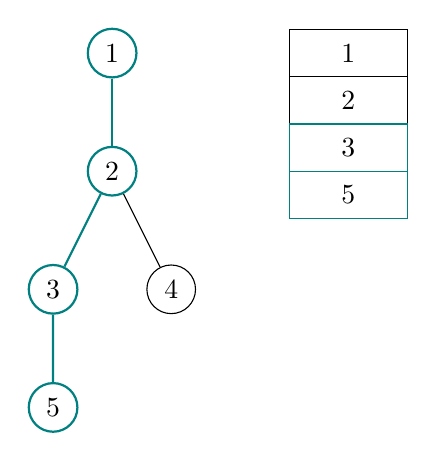
\begin{tikzpicture}

% the tree

\begin{scope}[circle,thick,draw=teal,every node/.style={draw}]
    \node at (0,0) {$1$}
        child {node {$2$}
            child {node {$3$}
                child {node {$5$}}}
            child[draw=black,thin] {node {$4$}}};
\end{scope}

% the stack

\begin{scope}[minimum height=6mm,minimum width=1.5cm,
        every node/.style={draw}]
    \node at (3cm,0mm) {$1$};
    \node at (3cm,-6mm) {$2$};
    \node[draw=teal] at (3cm,-12mm) {$3$};
    \node[draw=teal] at (3cm,-18mm) {$5$};
\end{scope}

\end{tikzpicture}
\end{document}
